\chapter{Operations at Sea and Field Work in Guaymas Basin}
%Preface that the intent of this chapter is to highlight practical engineering necessities and opportunities for deep sea research.

\begin{center}
    \begin{minipage}{0.5\textwidth}
      \begin{small}
        How inappropriate to call this planet Earth when it is quite clearly Ocean.\\ \emph{Arthur C. Clarke}
      \end{small}
    \end{minipage}
    \vspace{0.5cm}
\end{center}

Field robotics is a subfield of research devoted to enabling sophisticated robotic autonomy or control directly within the environmental and task contexts for which they were designed.
Being a field roboticist means developing sophistication with practicalities in mind.
Practicalities in the case of launching expeditionary robots may include the location and nature of the deployment site, the support infrastructure necessary for robot deployment and human life-support, and managing expectations between multiple on-site stakeholders.
In this thesis, a field deployment in the Guaymas Basin, Gulf of California serves as the grounding context for a deployment of AUV \Sentry to chart hydrothermal plumes.
This chapter will provide a general overview of field operations for this context, with detailed discussion of the philosophy of robotics in this setting....
\td{this needs updated once content is more in place}

\section{Overview of the Guaymas Basin Setting}
\label{sec:field_description}
In November 2021, research cruise RR2107 aboard the research vessel (R/V) \emph{Roger Revelle} was conducted at the Guaymas Basin in the Gulf of California (Mexico). A mid-ocean ridge extensional spreading center, there has been a long documented history of hydrothermal expressions in the Guaymas Basin, with a particular focus on the southern basin\footnote{e.g., \autocite{ondreas2018recent, teske2016guaymas, seewald1994variations, von1985chemistry, lonsdale1985hydrothermal}}. RR2107 was uniquely focused on studying two northern basin sites, the Northern Ridge and Ring Vent, with several key objectives: test novel \emph{in situ} instruments to measure dissolved methane\autocite{kapit2021dissolved,kapit2021measurement,michel2022gas}, test novel \emph{in situ} instruments to measure the carbonate cycle, map the heat distribution in shallow sediments above hydrothermal sills, collect tubeworm and geological specimens, and collect biological samples of microbiota in hydrothermal plume-fluids to re-construct the structure of a plume microbiome. It is typical that research cruises have several science teams working together under an appointed chief scientist to maximize the use of ship assets while at sea, and this cruise was no exception. To enable science operations, AUV \Sentry, remotely-operated vehicle (ROV) \emph{JASON}, and standard oceanographic equipment (i.e., Conductivity-Temperature-Depth (CTD) rosette, Niskin carousel, shipboard acoustics) were available. The deployment of autonomy on the cruise for \Sentry operations was coupled with objectives to test \emph{in situ} instruments and collect microbiota samples. For both of these tasks, charting different regions within a plume was important to test the capabilities of the novel instruments and collect biological samples from a diversity of plume-conditions.


Ring Vent is a diffusive venting site\autocite{teske2019characteristics}, so \Sentry studies for the purposes of this thesis were primarily conducted at the Northern Ridge. The Northern Ridge is a recently discovered hydrothermal site\autocite{soule2018exploration, geilert2018formation}, approximately \SI{1850}{\meter} underwater and at the edge of an additionally \SI{300}{\meter} deeper graben (a valley with steep sides) (\cref{fig:site}). The ridge is approximately \SI{600}{\meter} long and features several tall sulfide structures 10-\SI{25}{\meter} in height with active smoking along their bodies. A smoking ``chimney'' at the northernmost point of the ridge was targeted for plume-charting. The chimney vent is composed of a cluster of tens of small orifices ($<$\SI{0.1}{\meter} diameter) that create an approximately \SI{1.5}{\meter} diameter chimney base. The fluid produced is thick with particulate matter and highly-enriched in carbon dioxide (CO$_2$), hydrogen (H$_2$), and methane (CH$_4$), among others. Measured with a temperature wand on \emph{JASON}, fluid temperature at the vent orifice is estimated to be \SI{340}{\celsius} and ventilate rapidly. In contrast, the ambient seawater is methane-poor, considerably less turbid, and cold at \SI{4}{\celsius}. As vent fluids rise and form a plume at this site, the ambient water mixes (entrains) at an unknown rate, and advects by mild deep-water currents. Under these conditions, plume expressions could be transported several hundred meters from a known source, and would be expected to rise over \SI{200}{\meter} in the water column\autocite{speer1989model}.


\begin{figure}[!ht]
    \centering
    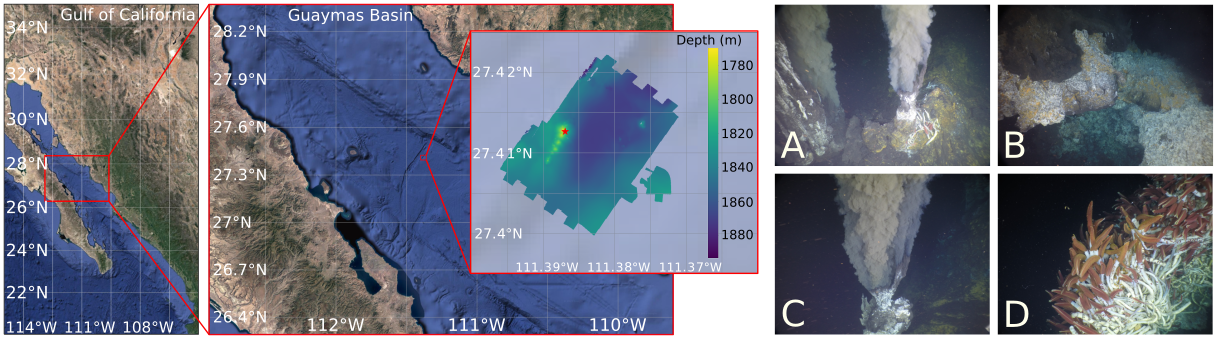
\includegraphics[width=\columnwidth]{figures/site_summary.png}
    \caption{\textbf{Autonomy study site in the Guaymas Basin, Gulf of California.} The inset map is bathymetric data collected by AUV \Sentry during RR2107 and shows the approximately \SI{600}{\meter} long ridge in yellow. The red star marks the chimney used as reference for autonomy studies. Pictures A-D show imagery from the ridge and chimney site. A-C show various forms of plume-producing vents located at the chimney and D shows an example of the macrofauna covering the structures along the ridge.}
    \label{fig:site}
\end{figure}
 

\section{Challenges for Robots in the Deep Ocean}
\label{sec:ops_challenges}
% No GPS, no satellite, only acoustics, very few observatories, etc.
In the Guaymas Basin setting, or any deep ocean research, there are several unique challenges to deploying robotic platforms in contrast to terrestrial applications. Perhaps the most quintessential of these challenges is the conductive nature of water, and its corresponding attenuation of radio frequencies\autocite{qureshi2016rf}. The natural consequence is that ubiquitous technologies like global position satellites (GPS), imaging satellites, and radio-based wireless communication are not available for underwater navigation, mapping, or communication. 

\section{Overview of Science Teams and Responsibilities}
Establish how computer scientists fit on a ship.

\section{Data Infrastructure on a Vessel}
Propose live-streaming\dots

\section{Taking Ground Truth Measurements}
Basically impossible, some things more than others.

\subsection{Water Column Standards}
Profiles gathered

\subsection{Hydrothermal Vents}

\subsubsection{Geochemical Measurements}
Jason wand/standard equipment

\subsubsection{Physical Measurements}
Fluid exit velocity, PIV system

\subsection{Crossflow}
Tiltmeters
